% Created 2021-09-28 Tue 15:49
% Intended LaTeX compiler: pdflatex
\documentclass{scrartcl}
\usepackage[utf8]{inputenc}
\usepackage[T1]{fontenc}
\usepackage{fontspec}
\usepackage{graphicx}
\usepackage{grffile}
\usepackage{longtable}
\usepackage{wrapfig}
\usepackage{rotating}
\usepackage[normalem]{ulem}
\usepackage{amsmath}
\usepackage{textcomp}
\usepackage{amssymb}
\usepackage{capt-of}
\usepackage[dvipsnames]{xcolor}
\usepackage[colorlinks=true, linkcolor=Blue, citecolor=BrickRed, urlcolor=PineGreen]{hyperref}
\usepackage{indentfirst}
\setmainfont[Ligatures=TeX]{Alegreya}
\setmonofont[Ligatures=TeX]{Liga SFMono Nerd Font}
% features: (acronym par-sep image table)
\newcommand{\acr}[1]{\protect\textls*[110]{\scshape #1}}
\newcommand{\acrs}{\protect\scalebox{.91}[.84]\hspace{0.15ex}s}
\setlength{\parskip}{\baselineskip}
\setlength{\parindent}{0pt}

\usepackage{graphicx}
\usepackage{longtable}
\usepackage{booktabs}
% end features

%% make document follow Emacs theme

\definecolor{obg}{HTML}{fafafa}
\definecolor{ofg}{HTML}{383a42}

\pagecolor{obg}
\color{ofg}

% list labels

\definecolor{itemlabel}{HTML}{4078f2}

\renewcommand{\labelitemi}{\textcolor{itemlabel}{\textbullet}}
\renewcommand{\labelitemii}{\textcolor{itemlabel}{\normalfont\bfseries \textendash}}
\renewcommand{\labelitemiii}{\textcolor{itemlabel}{\textasteriskcentered}}
\renewcommand{\labelitemiv}{\textcolor{itemlabel}{\textperiodcentered}}

\renewcommand{\labelenumi}{\textcolor{itemlabel}{\theenumi.}}
\renewcommand{\labelenumii}{\textcolor{itemlabel}{(\theenumii)}}
\renewcommand{\labelenumiii}{\textcolor{itemlabel}{\theenumiii.}}
\renewcommand{\labelenumiv}{\textcolor{itemlabel}{\theenumiv.}}

% structural elements

\definecolor{documentTitle}{HTML}{a626a4}
\definecolor{documentInfo}{HTML}{a626a4}
\definecolor{level1}{HTML}{e45649}
\definecolor{level2}{HTML}{da8548}
\definecolor{level3}{HTML}{b751b6}
\definecolor{level4}{HTML}{6f99f5}
\definecolor{level5}{HTML}{bc5cba}
\definecolor{level6}{HTML}{9fbbf8}
\definecolor{level7}{HTML}{d292d1}
\definecolor{level8}{HTML}{d8e4fc}

\addtokomafont{title}{\color{documentTitle}}
\addtokomafont{author}{\color{documentInfo}}
\addtokomafont{date}{\color{documentInfo}}
\addtokomafont{section}{\color{level1}}
\newkomafont{sectionprefix}{\color{level1}}
\addtokomafont{subsection}{\color{level2}}
\newkomafont{subsectionprefix}{\color{level2}}
\addtokomafont{subsubsection}{\color{level3}}
\newkomafont{subsubsectionprefix}{\color{level3}}
\addtokomafont{paragraph}{\color{level4}}
\newkomafont{paragraphprefix}{\color{level4}}
\addtokomafont{subparagraph}{\color{level5}}
\newkomafont{subparagraphprefix}{\color{level5}}

% textual elements

\definecolor{link}{HTML}{4078f2}
\definecolor{cite}{HTML}{4aa8b0}
\definecolor{itemlabel}{HTML}{4078f2}
\definecolor{code}{HTML}{da8548}
\definecolor{verbatim}{HTML}{50a14f}

\renewcommand{\labelitemi}{\textcolor{itemlabel}{\textbullet}}
\renewcommand{\labelitemii}{\textcolor{itemlabel}{\normalfont\bfseries \textendash}}
\renewcommand{\labelitemiii}{\textcolor{itemlabel}{\textasteriskcentered}}
\renewcommand{\labelitemiv}{\textcolor{itemlabel}{\textperiodcentered}}

\renewcommand{\labelenumi}{\textcolor{itemlabel}{\theenumi.}}
\renewcommand{\labelenumii}{\textcolor{itemlabel}{(\theenumii)}}
\renewcommand{\labelenumiii}{\textcolor{itemlabel}{\theenumiii.}}
\renewcommand{\labelenumiv}{\textcolor{itemlabel}{\theenumiv.}}

\DeclareTextFontCommand{\texttt}{\color{code}\ttfamily}
\makeatletter
\def\verbatim@font{\color{verbatim}\normalfont\ttfamily}
\makeatother

% code blocks

\definecolor{codebackground}{HTML}{f6f6f6}
\colorlet{EFD}{ofg}
\definecolor{codeborder}{HTML}{f0f0f0}

%% end customisations

\author{Shaurya Singh}
\date{\today}
\title{Graphing HW \#1\\\medskip
\large Biology I}
\colorlet{greenyblue}{blue!70!green}
\colorlet{blueygreen}{blue!40!green}
\providecolor{link}{named}{greenyblue}
\providecolor{cite}{named}{blueygreen}
\hypersetup{
  pdfauthor={Shaurya Singh},
  pdftitle={Graphing HW \#1},
  pdfkeywords={},
  pdfsubject={},
  pdfcreator={Emacs 28.0.50 (Org mode 9.5)},
  pdflang={English},
  breaklinks=true,
  colorlinks=true,
  linkcolor=,
  urlcolor=link,
  citecolor=cite
}
\urlstyle{same}
\begin{document}

\maketitle
\setcounter{tocdepth}{2}
\tableofcontents


\section{Pre-Lab Discussion}
\label{sec:orgf5d7f80}
\begin{enumerate}
\item Would a line graph or a bar graph be better for showing the number of birds
of each color in a population?
\begin{itemize}
\item A Bar Graph would be better, as the data is grouped data.
\end{itemize}
\item How could you plot more than one responding variable on a line graph?
\begin{itemize}
\item You could plot two lines on one graph.
\end{itemize}
\item Where do you place the manipulated variable on a line graph?
\begin{itemize}
\item The manipulated (independant) variable goes on the X-axis.
\end{itemize}
\item Which type of graph would you use to show comparisons? Explain the reason for your answer.
\begin{itemize}
\item I would use a Pie Chart, as its effective in showing parts of a whole. If
you wan't a precise comparison (as opposed to a relative one), use a bar graph
\end{itemize}
\item Why is it important to have all parts of a graph clearly labeled and drawn?
\begin{itemize}
\item Graphs that are clearly labeled are much less likely to be misread or misinterpreted.
\end{itemize}
\end{enumerate}

\section{Procedure}
\label{sec:org65f2263}
\subsection{Part A: Interpreting Graphs}
\label{sec:orgbf10e98}
\begin{enumerate}
\item No answer required
\item Use the line graph in Figure 2 to answer the following questions
\begin{enumerate}
\item Which plant grew the tallest
\begin{itemize}
\item Plant 2
\end{itemize}
\item How many plants grew to be at least 6 cm tall?
\begin{itemize}
\item All 3 plants grew to be atleast 6cm tall
\end{itemize}
\item Which plant grew the fastest in the first five days?
\begin{itemize}
\item Plant 3 grew the fastest the first 5 days
\end{itemize}
\item Which line represents plant 2?
\begin{itemize}
\item The dotted (----) line represents plant 2
\end{itemize}
\item After 10 days, how much had plant 3 grown?
\begin{itemize}
\item After 10 days plant 3 was 6cm tall
\end{itemize}
\item How long did it take for plant 1 to grow 6 cm?
\begin{itemize}
\item It took 15 days for plant 1 to reach 6cm
\end{itemize}
\end{enumerate}
\item No answer required
\item Use the bar graph to answer the following questions
\begin{enumerate}
\item At birth, what is the average number of red blood cells per mm of blood?
\begin{itemize}
\item At birth, there are 5.7 million blood cells/mm\(^{3}\) on average
\end{itemize}
\item What appears to happen to the number of red blood cells between birth and 2 months?
\begin{itemize}
\item The number of red blood cells drastically decresaes between birth and 2 months
\end{itemize}
\item What happens to the number of red blood cells between the ages of 6 and 8 years?
\begin{itemize}
\item From 6 to 8 years, the number of red blood cells stays the same
\end{itemize}
\item Between what ages is a human likely to have 4.6 million red blood cells?
\begin{itemize}
\item Someone is likely to have 4.6 million red blood cells from 6-12 months of age
\end{itemize}
\item After 14 years of age, do males or females have a higher red blood cell count?
\begin{itemize}
\item After 14 years of age, males have a higher blood cell count
\end{itemize}
\end{enumerate}
\end{enumerate}

\subsection{Part B: Constructing Graphs}
\label{sec:orgee9a868}
\subsubsection{Data Table 1:}
\label{sec:orged790f0}
Use the information recorded in Data Table 1 to construct a line
graph on the grid provided below. You should label each axis, mark an appropriate scale on each axis, plot the data, connect the points,
and give your graph a title

\begin{center}
\begin{tabular}{rr}
\toprule
Temperature(C) & Breathing Rate (Per Minute)\\
\midrule
10 & 15\\
\midrule
15 & 25\\
\midrule
18 & 30\\
\midrule
38 & 60\\
\midrule
57 & 25\\
\bottomrule
\end{tabular}
\end{center}

\begin{center}
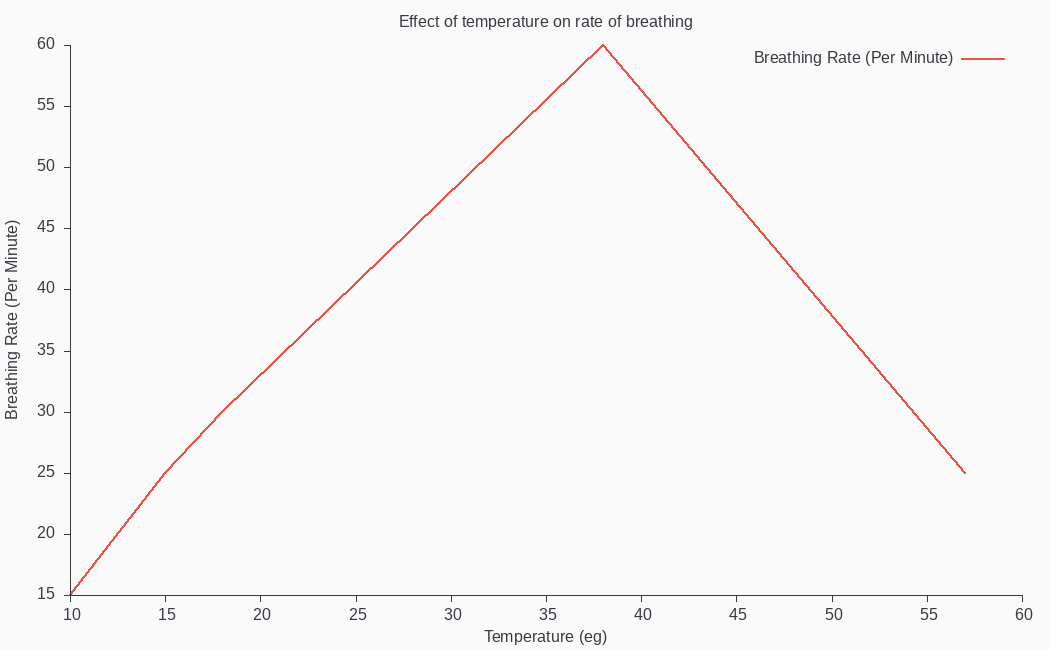
\includegraphics[width=.9\linewidth]{./temperatureVSbreathing.jpeg}
\end{center}

\subsubsection{Data Table 2:}
\label{sec:org95e81b0}
Use the information recorded in Data Table 2 to construct a bar graph
on the grid provided below. You should label each axis, mark an appropriate
scale on each axis, plot the data, darken the columns of the graph, and give
your graph a title.

\begin{center}
\begin{tabular}{lr}
\toprule
Month & Rainfall (mL)\\
\midrule
Jan. & 15\\
Feb. & 21\\
Mar. & 28\\
April & 24\\
May & 16\\
June & 8\\
July & 2\\
Aug. & 1\\
Sept & 2\\
Oct. & 3\\
Nov. & 5\\
Dec. & 10\\
\bottomrule
\end{tabular}
\end{center}

\begin{center}
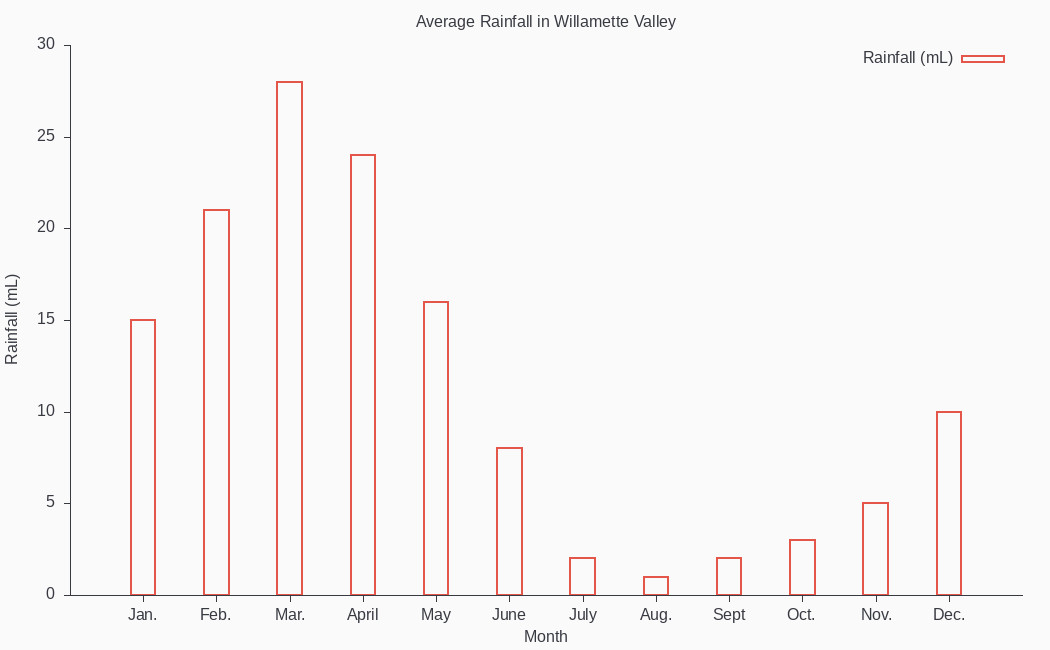
\includegraphics[width=.9\linewidth]{./averagerainfall.jpeg}
\end{center}

\section{Analysis and Conclusions}
\label{sec:org7f9a7f8}
\begin{enumerate}
\item \textbf{Comparing and Contrasting:} How is a graph similar to a data table?
\begin{itemize}
\item Graphs and table are similar because they both present the evidential and
statistic data given and yielded from a certain experiment or testing. They
both have a role in classification, categorization, interpretation and
organization of the data. A table presents the raw data, while a graph
visualizes it
\end{itemize}

\item \textbf{Comparing and Contrasting:} How is a line graph different from a bar graph?
\begin{itemize}
\item Bar graphs show data with blocks of different lengths, whereas line graphs
show a series of points connected by straight lines. Bar graphs are more
versatile while line graphs are better for showing trends over time or
another measure with a logical progression of values. Bar graphs can also
show frequency distributions much more effectively than line graphs.
\end{itemize}

\item \textbf{Using Graphs:} Does a steep curve on a line graph indicate a rapid or slow
rate of change?
\begin{itemize}
\item A steep curve on a line graph would indicate a rapid rate of change
\end{itemize}

\item \textbf{Using Graphs:} You are conducting an experiment to measure the gain in mass of
a young mouse over a ten-week period. In constructing a graph to represent
your data, which variable should you place along the x-axis and which
variable should you place along the y-axis? Explain your answer.
\begin{itemize}
\item On the x-axis you would put the independent/manipulated variable, which is
the time. On the y-axis is the dependant variable, which is the gain in
mass.
\end{itemize}

\item \textbf{Using Graphs:} What is an advantage of using multiple lines in a line graph?
(See Figure 2.)
\begin{itemize}
\item With multiple lines, you can display multiple sets of data, allowing the
reader to easily compare and contrast the datasets.
\end{itemize}
\end{enumerate}
\end{document}
